\documentclass[tikz, border=10pt]{standalone}
\usepackage{graphicx}
\usepackage{amsmath,amssymb,amsfonts}
\usepackage{changepage}
\usepackage{tabularx,booktabs}
\usepackage{multirow}
\usepackage{subcaption}
\tikzset{
    vertex/.style = {
        circle,
        fill            = black,
        outer sep = 2pt,
        inner sep = 1pt,
    }
}
\begin{document}
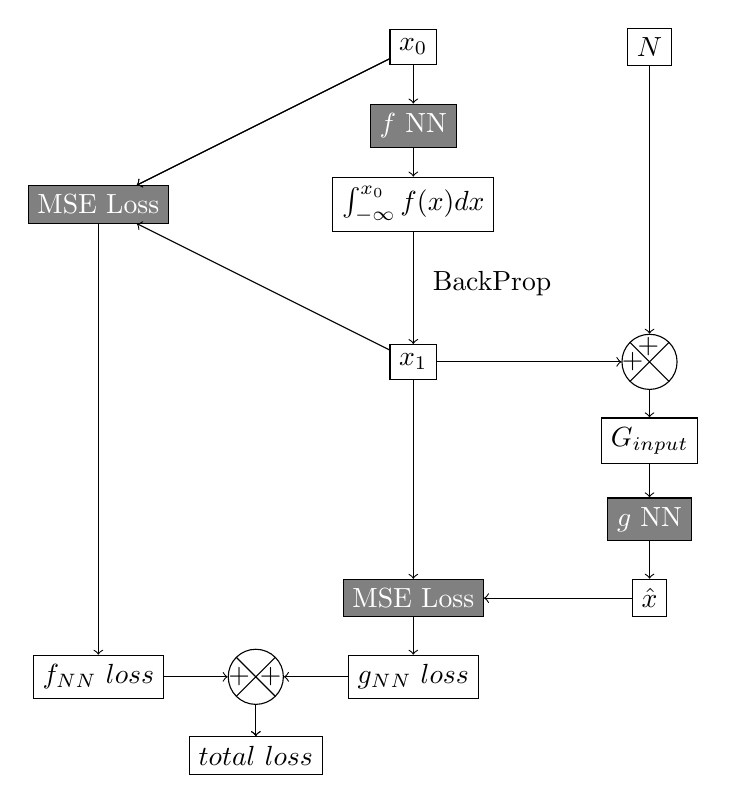
\begin{tikzpicture}[cross/.style={path picture={ 
    \draw[black]
  (path picture bounding box.south east) -- (path picture bounding box.north west) (path picture bounding box.south west) -- (path picture bounding box.north east);
  }}]
  % Dialectics
  \node[draw] (x0) at (0,10) {$x_0$};
  \node[draw] (N) at (3,10) {$N$};
%   \node[draw] (x0) at (0,8) {Variable($x_0$)};
  \node[draw,,fill=gray,text=white] (fNN) at (0,9) {$f$ NN};
%   \node[draw,,fill=gray,text=white] (gNN) at (3,9) {$g$ NN};
  
  \node[draw] (integralx1) at (0,8) {$\int_{-\infty}^{x_0} f(x) dx$};

  \node[draw] (x1) at (0,6) {$x_1$};

% Draw the summation
  \node [draw,circle,cross,minimum width=0.7 cm](sum) at (3,6){};
  \node [text width=0.7 cm]at (3,6){+};
  \node [text width=0.7 cm]at (3.2,6.2){+}; 

  \node[draw] (Gin) at (3,5) {$G_{input}$};

  \node[draw,,fill=gray,text=white] (gNN) at (3,4) {$g$ NN};
  \node[draw] (xhat) at (3,3) {$\hat x$};

\node[draw,fill=gray,text=white] (MSE2) at (0,3) {MSE Loss};
\node[draw,fill=gray,text=white] (MSE1) at (-4,8) {MSE Loss};

\node[draw] (gloss) at (0,2) {$g_{NN}$ $loss$};
\node[draw] (floss) at (-4,2) {$f_{NN}$ $loss$};

% Draw the summation
\node [draw,circle,cross,minimum width=0.7 cm](sumloss) at (-2,2){};
\node [text width=0.7 cm]at (-2,2){+};
\node [text width=0.7 cm]at (-1.6,2){+}; 

\node[draw] (totalloss) at (-2,1) {$total$ $loss$};

 \node at (1, 7) {Back\\Prop};
 \draw[->] (x0)--(fNN);
% \draw[->] (integralx1)-- (x1);
\draw[->](fNN)--(integralx1);
\draw[->](integralx1)--(x1);
\draw[->](x1)--(sum);
\draw[->](N)--(sum);
\draw[->](sum)--(Gin);
\draw[->](Gin)--(gNN);
\draw[->](gNN)--(xhat);
\draw[->](xhat)--(MSE2);
\draw[->](x1)--(MSE2);
\draw[->](MSE2)--(gloss);
\draw[->](gloss)--(sumloss);
\draw[->](sumloss)--(totalloss);
\draw[->](x0)--(MSE1);
\draw[->](x1)--(MSE1);
\draw[->](MSE1)--(floss);
\draw[->](floss)--(sumloss);
\draw[->](sumloss)--(totalloss);
\draw[->](x0)--(MSE1);


%   \draw[->] (x0)--(fNN)--(integralx1)--(x1)--(sum);
%   \draw[->] (N)--(sum)--(Gin)--(gNN)--(xhat)--(MSE2);
%   \draw[->] (x1)--(MSE2)--(gloss)--(sumloss);
%   \draw[->] (x1)--(MSE1)--(floss)--(sumloss)--(totalloss);
%   \draw[->] (x0)--(MSE1);


%   \draw[->,draw=blue] (Synthesis) to[in=180,out=180] (x0);
  

\end{tikzpicture}
\end{document}